\documentclass{./../div_teaching_slides}
\usepackage{setspace}

\begin{document}
\title{ECON 340 \\ Economic Research Methods}
\author{Div Bhagia \\\vspace{1.75em}
Lecture 3 \\\vspace{0.25em} \small Variance, Standard Deviation, Z-Score}
\date{}

\begin{frame}[noframenumbering, plain]
\maketitle
\end{frame}

%%%%%%%%%%%%%%%%%%%%
\begin{frame}{NYT Article: 2016 Election Predictions}
\begin{witemize}
  \item Summarize the main issue being discussed in the article.
  \item What were the three types of errors identified in the article? What is the common thread across these errors?
  \item One of the fixes suggested in the article was ``education weighting''. Which of the three errors would this fix and how? \pause 
  \item In general, how can we pick a sample that is representative of the population to avoid having to reweight?
\end{witemize}
\end{frame}

%%%%%%%%%%%%%%%%%%%%
\begin{frame}{Another Example}
\vspace{-0.5em}
\begin{witemize}
	\item We want to estimate the average starting salary of students at a university that has only two majors	\item Half of the students are \textit{Business} majors, while the other half are \textit{Engineering} majors
	\item Randomly select 100 Business students and 100 Engineering for a survey
	\item Response rate among Business students is 100\%, while it 50\% for engineering students 
	\item[] \textit{How can we use weighting to adjust for this?}
\end{witemize}
\end{frame}	

%%%%%%%%%%%%%%%%%%%%
\begin{frame}{Last Class}
How to describe variables? \\~\\
\begin{witemize}
  \item Empirical Distribution
  \item Measures of central tendency: mean and median \\~\\
\end{witemize}
$\mu:$ population mean, $\bar{X}:$ sample mean \\~\\
Two equivalent formulas:
$$ \bar{X} = \frac {\sum_{i=1}^n X_i}{n} \quad \quad \quad \quad \bar{X} = \sum_{k=1}^K f_k X_k $$
\end{frame}

%%%%%%%%%%%%%%%%%%
\begin{frame}{Measures of central tendency are not enough!}
\centering \vspace{-0.5em}
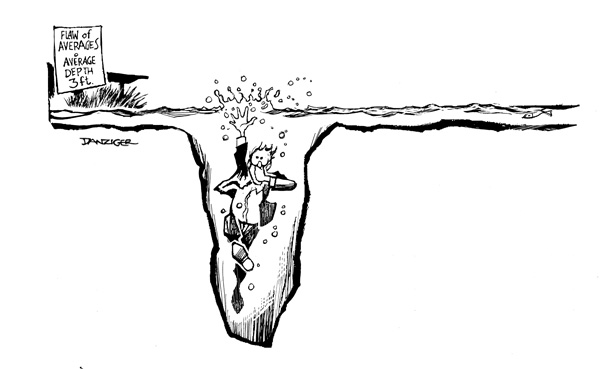
\includegraphics[scale=0.525]{flaw}
\end{frame}

%%%%%%%%%%%%%%%%%%
\begin{frame}{Where would you want to live?}
\centering
\begin{tabular}{cc}
Mushroom Kingdom  & Bowser's Kingdom \\
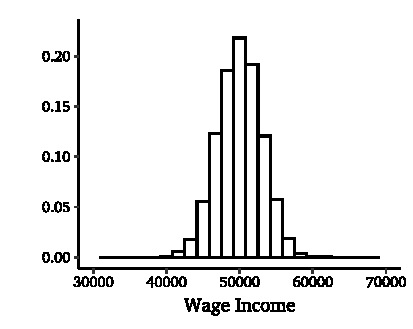
\includegraphics{./../../Output/income_mk.pdf} &
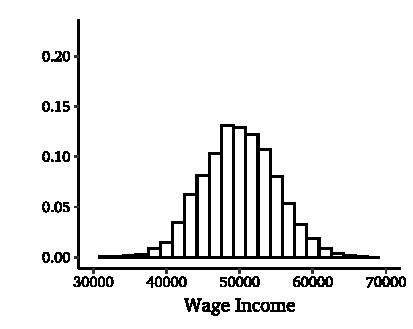
\includegraphics{./../../Output/income_bk.pdf} \\
Mean = Median= \$50,000 & Mean = Median= \$50,000 \\
\end{tabular}
\end{frame}

%%%%%%%%%%%%%%%%%%
\begin{frame}{Deviations from the Mean}
\begin{witemize}
  \item Even with identical mean and median, the two countries are not identical. 
  \item There is certainly more \textit{dispersion} or \textit{variability} in income in Bowser's Kingdom. 
  \item More observations are \textit{further from the mean} in Bowser's Kingdom. 
  \item \textit{What could be a potential statistic that could capture this?}
\end{witemize}
\end{frame}

%%%%%%%%%%%%%%%%%%
\begin{frame}{Deviations from the Mean}
 One option: average deviations from the mean. \textit{Will this work?} \\~\\
 \setstretch{1.25}
  \begin{tabularx}{0.5\textwidth}{|P{1.25cm}|Y|}
  \hline
  $X_i$ & $X_i-\mu$ \\
  \hline
  5 & \\
  \hline
  5 & \\
  \hline
  10 & \\
  \hline
  10 & \\
  \hline
  20 & \\
  \hline
   & \\
  \hline
  \end{tabularx}
\end{frame}

%%%%%%%%%%%%%%%%%%
\begin{frame}{Deviations from the Mean}
Why does this not work? Remember from the last class:
\begin{align*}
 \sum_{i=1}^n (X_i - \bar{X}) &=  \sum_{i=1}^n X_i - \sum_{i=1}^n \bar{X} \quad \quad (Why?) \\
 &=  \sum_{i=1}^n X_i - n \bar{X} \\
 &=  n \bar{X} - n \bar{X} = 0 \quad \quad (Why?) 
 \end{align*} 
 \vspace{0.25em}
 
 \pause
 \textit{Can you think of a way to construct a statistic that would capture variation around the mean?}
\end{frame}

%%%%%%%%%%%%%%%%%%
\begin{frame}{Variance and Standard Deviation }
\textit{Population Variance}
$$ \sigma_X^2 = \frac{1}{N} \sum_{i=1}^N (X_i-\mu_x)^2 $$
\textit{Sample Variance}
$$ S_X^2 = \frac{1}{n-1} \sum_{i=1}^n (X_i-\bar{X})^2 $$
\textit{Standard Deviation}
$$ \sigma_X = \sqrt{\sigma_X^2} \quad \quad S_X = \sqrt{S_X^2} $$
\end{frame}

%%%%%%%%%%%%%%%%%%
\begin{frame}{Variance and Standard Deviation}
Back to our example. \\~\\
 \setstretch{1.25}
  \begin{tabularx}{0.6\textwidth}{|P{1.5cm}|Y|Y|}
  \hline
  $X_i$ & $(X_i-\mu)$ & $(X_i-\mu)^2$ \\
  \hline
  5 & -5 & \\
  \hline
  5 & -5 & \\
  \hline
  10 & 0 & \\
    \hline
  10 & 0 & \\
    \hline
  20 & 10& \\
  \hline
 \textbf{50}  & \textbf{0} & \\
  \hline
  \end{tabularx}
\end{frame}

%%%%%%%%%%%%%%%%%%%%
\begin{frame}{Variance with Grouped Data}
\textit{Population Variance}
$$ \sigma_X^2 = \sum_{k=1}^K f_k (X_k-\mu_X)^2 $$
\textit{Sample Variance}
 $$ S_X^2 = \frac{n}{n-1} \sum_{k=1}^K f_k (X_k-\bar{X})^2 $$
\end{frame}

%%%%%%%%%%%%%%%%%%
\begin{frame}{Variance with Grouped Data}
In our example: 5, 5, 10, 10, 20. Present this as: \\~\\
 \setstretch{1.25}
  \begin{tabularx}{\textwidth}{|P{1.5cm}|P{1.5cm}|P{1.5cm}|Y|Y|}
  \hline
  $X_k$ & $f_k$ & $f_k X_k $ & $(X_k-\mu)^2$ & $f_k (X_k-\mu)^2$ \\
  \hline
  5 & 2/5 &  & & \\
  \hline
  10 & 2/5 &  &  & \\
  \hline
  20 & 1/5 &  & & \\
  \hline
 Total  &  &  & & \\
  \hline
  \end{tabularx}
\end{frame}

%%%%%%%%%%%% 
\begin{frame}{Where would you want to live?}
\centering \vspace{-0.5em}
\begin{tabular}{cc}
Mushroom Kingdom  & Bowser's Kingdom \\
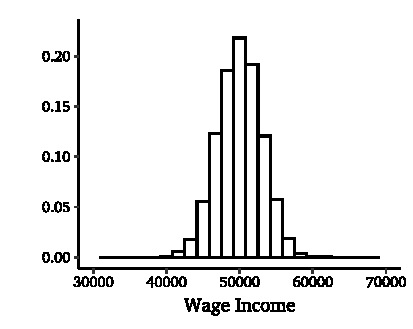
\includegraphics{./../../Output/income_mk.pdf} &
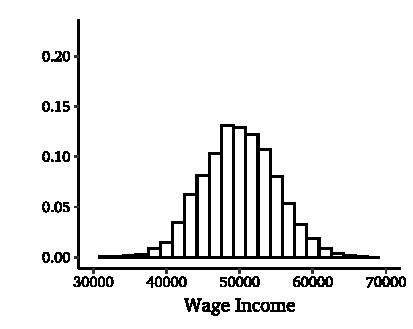
\includegraphics{./../../Output/income_bk.pdf} \\ 
Mean = Median= \$50,000 & Mean = Median= \$50,000 \\
SD= \$3,000 & SD= \$5,000 \\
\end{tabular}
\end{frame}

%%%%%%%%%%%%
\begin{frame}{Where would you want to live?}
\begin{witemize}
  \item If we don't know where we will end up in the income distribution, some of us might prefer the Mushroom Kingdom since it is unlikely we would earn very little. 
  \item For the same reason, some of us might like Bowser, as it is more likely that one could make a lot.
  \item But what if Luigi has a job for you as a plumber in both locations, and you will earn \$45,000 regardless of where you end up? Are you now indifferent between the two?
\end{witemize}
\end{frame}

%%%%%%%%%%%% 
\begin{frame}{Where would you want to live?}
\centering \vspace{-0.5em}
\begin{tabular}{cc}
Mushroom Kingdom  & Bowser's Kingdom \\
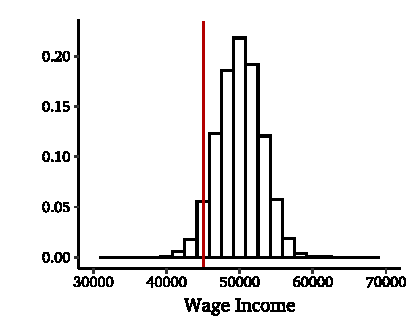
\includegraphics{./../../Output/income_mk_z.pdf} &
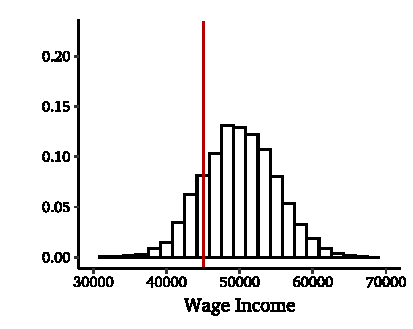
\includegraphics{./../../Output/income_bk_z.pdf} \\ 
Mean = Median= \$50,000 & Mean = Median= \$50,000 \\
SD= \$3,000 & SD= \$5,000 \\
\end{tabular}
\end{frame}

%%%%%%%%%%%% 
\begin{frame}{Z-Score}
We can calculate the Z-Score to capture how many standard deviations ($\sigma$) away from the mean ($\mu$) a specific observation is. \\
$$ Z = \frac{X - \mu}{\sigma} \quad \rightarrow \quad X = \mu + Z.\sigma $$ \\~\\


Example: $\sigma_{MK} = 3000$, $\sigma_{BK} = 5000$ \\
 $$Z_{MK} = \frac{45000 - 50000}{3000} = -1.66 \quad \quad Z_{BK} = \frac{45000 - 50000}{5000} = -1$$ \\~\\
\end{frame}

%%%%%%%%%%%% 
\begin{frame}{Z-Score}
\begin{witemize}
\item Someone who earns \$45,000 in the Mushroom Kingdom is 1.66 \textit{standard deviations} below the mean.
\item While someone who earns \$45,000 in the  Bowser's Kingdom is $1$ \textit{standard deviation} below the mean.
  \item Here, Z-score is informative about how many people are there between someone who earns \$45,000 and the average person 
  \item More generally, Z-score tells us the relative position of an observation in the distribution
\end{witemize}
\end{frame}

%%%%%%%%%%%%%%%%%%%%
\begin{frame}{Things to do next}
\begin{witemize}
\item Make sure you are staying up to date with the class; notes complement the slides
\item Please utilize my office hours
\item Start thinking about your research partner \vspace{0.5em}
\begin{mitemize}
  \item You can self-sign up on Canvas by going to \textit{People} and then clicking on the \textit{Research Project Group} tab or email me
\item If you do not inform me of your partner or indicate that you will be working alone by Thurs Feb 6, I will assign a partner for you.
\end{mitemize}
\item Coming up: Problem Set 1 (due next week on Tues)
\end{witemize}
\end{frame}

\end{document}